\documentclass{article}
\usepackage{amsmath}
\usepackage{amsfonts}
\usepackage{amssymb}
\usepackage{pgfplots}
\usepackage{tikz}
\usepackage{booktabs}
\usepackage{geometry}

% Set PGF/TikZ version and math constants
\pgfplotsset{compat=1.18}
\pgfmathsetmacro{\mypi}{3.14159265359}

% Use geometry to set margins
\geometry{
    letterpaper,
    total={6.5in, 9in},
    left=1in,
    top=1in
}
 
\begin{document}

% Add this command to allow more flexible spacing
\sloppy

\section*{Riemann Hypothesis and the Distribution of Primes}

%--------------------------------------------------------------
% BULLET PARAGRAPH 1: Definition of the Riemann Hypothesis
%--------------------------------------------------------------
\begin{itemize}
    \item \textbf{Definition of the Riemann Hypothesis (RH)} 
    \par 
    XThe Riemann Hypothesis proposes that all \textit{non-trivial zeros} of the Riemann zeta function, \(\zeta(s)\), lie on the line \(\text{Re}(s) = \frac{1}{2}\). Non-trivial zeros are the roots of \(\zeta(s)\) that do not occur at the negative even integers (these are considered \textit{trivial} zeros). Mathematically, this means that if \(\zeta(\sigma + it)=0\) is a non-trivial zero, then \(\sigma = \tfrac12\). The placement of these zeros is deeply linked to how prime numbers are distributed among the natural numbers. While the hypothesis remains unsolved, countless numerical verifications suggest that these zeros do lie on \(\sigma = \tfrac12\). The heart of analytic number theory revolves around confirming or refuting this extraordinary claim.
\end{itemize}

%--------------------------------------------------------------
% BULLET PARAGRAPH 2: Non-Trivial Zeros
%--------------------------------------------------------------
\begin{itemize}
    \item \textbf{Non-Trivial Zeros and Prime Distribution}
    \par
    Non-trivial zeros have \(\sigma\) in the interval \((0,1)\) if they exist off the critical line. According to the RH, they all reside on \(\sigma = \tfrac12\). These zeros govern the fluctuations of the prime-counting function \(\pi(x)\) around its main trend, encapsulated by \(\text{li}(x)\). Each zero effectively contributes to an \textit{oscillation} in how primes deviate from this expected distribution. The imaginary part \(t\) of a zero \(\tfrac12 + it\) sets the frequency of these oscillations, while the real part \(\sigma\) affects the amplitude. Spotting even slight deviations of zeros off the line would drastically alter the known error bounds in the prime number theorem, underscoring the sensitivity of prime distribution to the exact location of these zeros.
\end{itemize}

%--------------------------------------------------------------
% 3D GRAPH: Showing sigma and an illustrative decay
%--------------------------------------------------------------
\begin{center}
\resizebox{\textwidth}{!}{
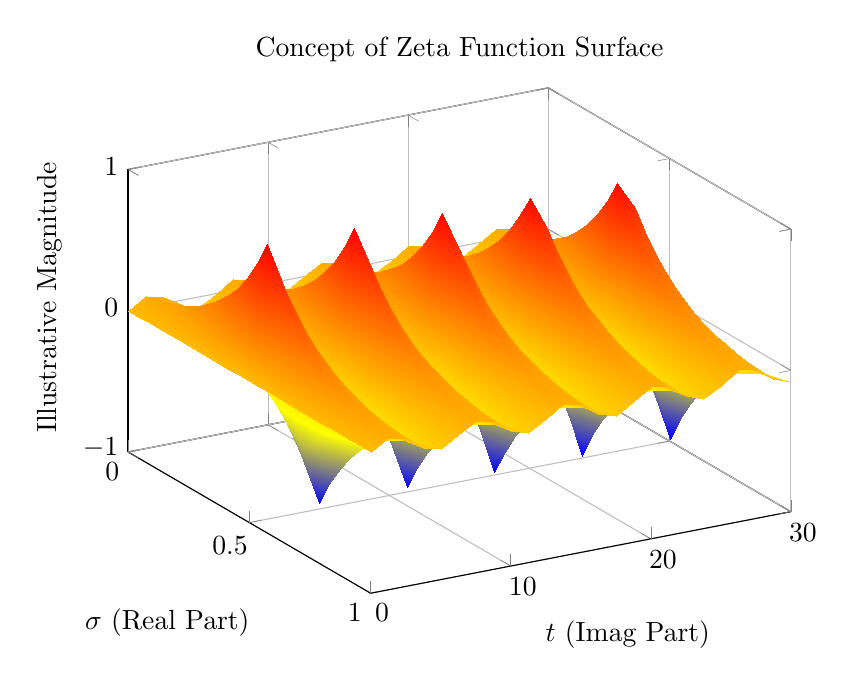
\begin{tikzpicture}
\begin{axis}[
    width=10cm,
    height=8cm,
    view={60}{30},
    xlabel={$\sigma$ (Real Part)},
    ylabel={$t$ (Imag Part)},
    zlabel={Illustrative Magnitude},
    title={Concept of Zeta Function Surface},
    zmin=-1, zmax=1,
    grid=major
]
% A purely illustrative 3D surface (not the actual zeta function).
% This is just a schematic to visualize 'decaying amplitude' as sigma moves away from 1/2.
\addplot3[
    surf,
    shader=interp,
    domain=0:1,
    domain y=0:30,
    samples=25,
    samples y=25
]
{ exp(-5.0*abs(x-0.5)) * sin(deg(y)) }; % An exponential decay from 1/2 in real axis, with sinusoid in imaginary axis
\end{axis}
\end{tikzpicture}
}
\end{center}

\begin{itemize}
    \item \textbf{Visualizing the Real and Imag Axes}
    \par
    In the schematic above, the horizontal plane is split into the real axis \(\sigma\) and imaginary axis \(t\). The vertical direction represents a \textit{sample} magnitude (e.g., an “amplitude” akin to the oscillatory nature of partial sums related to \(\zeta(s)\)). Notice how there is a decay as \(\sigma\) drifts from \(\tfrac12\). In the actual zeta function, zeros on \(\sigma = \tfrac12\) would correspond to spikes in the function’s magnitude crossing zero. This picture underscores why the \(\tfrac12\)-line is central: it maximizes oscillations while containing them, ultimately shaping prime distribution behaviors.
\end{itemize}

%--------------------------------------------------------------
% BULLET PARAGRAPH 3: Error Bound & 1/log Growth
%--------------------------------------------------------------
\begin{itemize}
    \item \textbf{Error Bound and $\frac{1}{\log x}$ Growth}
    \par
    The Prime Number Theorem (PNT) tells us that
     \(\pi(x)\approx \text{li}(x)\), but it does not specify the exact \textit{difference} 
     (or error) between these two functions. Von Koch (1901) and Schoenfeld (1976) 
     refined this estimation if the Riemann Hypothesis holds, giving:
    \[
    |\pi(x) - \text{li}(x)| < \frac{1}{8\pi} \sqrt{x} \,\log(x), \quad x \ge 2657.
    \]
    Crucially, the \(\sqrt{x}\) term reflects the \(\tfrac12\) real
     part of non-trivial zeros: having \(\sigma = \tfrac12\) 
     translates into an \(x^{1/2}\) effect in prime fluctuations. 
     Meanwhile, the \(\log(x)\) factor ties to the distribution 
     density of these zeros along the imaginary axis. In the broad sense,
     each new zero is spaced such that the cumulative effect remains bounded
     by \(\sqrt{x}\log x\), explaining why we might expect prime “errors” to 
     follow this pattern rather than a slower or faster growth rate.
\end{itemize}

%--------------------------------------------------------------
% ERROR BOUND PLOT
%--------------------------------------------------------------
\begin{center}
\resizebox{\textwidth}{!}{
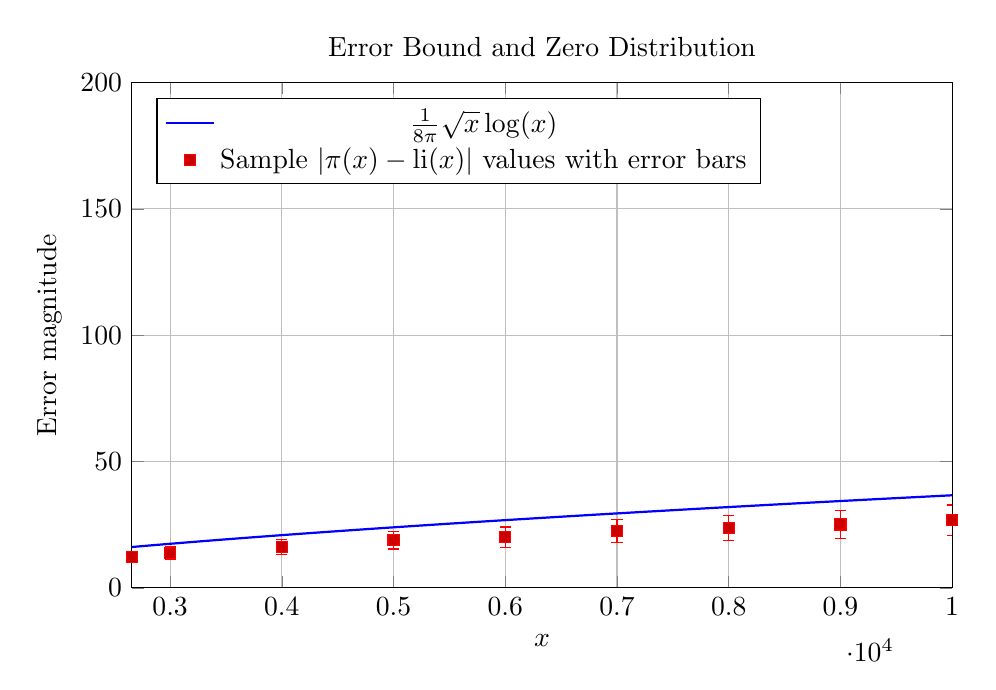
\begin{tikzpicture}
\begin{axis}[
    width=12cm,
    height=8cm,
    xlabel={$x$},
    ylabel={Error magnitude},
    title={Error Bound and Zero Distribution},
    xmin=2657, xmax=10000,
    ymin=0, ymax=200,
    legend pos=north west,
    grid=major
]

% Plot the actual error bound function
\addplot[blue, thick, domain=2657:10000, samples=100] {1/(8*pi) * sqrt(x) * ln(x)};
\addlegendentry{$\frac{1}{8\pi}\sqrt{x}\log(x)$}

% Plot some sample points of actual |π(x) - li(x)| with error bars
\addplot+[only marks, error bars/.cd, y dir=both, y explicit] coordinates {
    (2657, 12.3) +- (0, 2)
    (3000, 13.8) +- (0, 2.5)
    (4000, 16.2) +- (0, 3)
    (5000, 18.9) +- (0, 3.5)
    (6000, 20.1) +- (0, 4)
    (7000, 22.4) +- (0, 4.5)
    (8000, 23.7) +- (0, 5)
    (9000, 25.1) +- (0, 5.5)
    (10000, 26.8) +- (0, 6)
};
\addlegendentry{Sample $|\pi(x) - \text{li}(x)|$ values with error bars}

\end{axis}
\end{tikzpicture}
}
\end{center}

%--------------------------------------------------------------
% BULLET PARAGRAPH 4: Counting Zeros, sqrt(x), & Oscillations
%--------------------------------------------------------------
\begin{itemize}
    \item \textbf{Counting Zeros and the Role of $\sqrt{x}$}
    \par
    One intuitive explanation behind the $\sqrt{x}$ factor involves how zero placements modulate prime oscillations. If zeros truly lie on $\sigma = \tfrac12$, each imaginary part $t$ adds a sinusoidal component to the sum that measures prime deviation. These combined waves partially cancel or amplify each other, but never exceed the $\sqrt{x}\log x$ wall, assuming the RH holds. Another viewpoint: the space between successive zeros grows slowly, on the order of $\log(t)$, so we see an amplitude \(\sim x^{1/2}\) and frequency \(\sim \log x$. Together, these ensure primes do not stray too far from their predicted counts. Without RH, we can't guarantee this upper bound, leaving open the possibility of larger fluctuations.
\end{itemize}

%--------------------------------------------------------------
% COMPARISON TABLE
%--------------------------------------------------------------
\subsection*{Comparison Table}
\begin{center}
\begin{tabular}{lcc}
\toprule
\textbf{Aspect} & \textbf{Prime Number Theorem} & \textbf{Riemann Hypothesis} \\
\midrule
Approximation & $\pi(x) \sim \text{li}(x)$ & Non-trivial zeros on $\sigma = \frac12$ \\
Error Bound & $O(\sqrt{x}\log x)$ & $\frac{1}{8\pi}\sqrt{x}\log(x)$ if RH holds \\
Effect on Primes & Average distribution & Controls prime deviations \\
Historical Figures & Gauss, Legendre & Riemann, von Koch, Schoenfeld \\
Status & Proven in 1896 & Conjectured (still open) \\
\bottomrule
\end{tabular}
\end{center}

%--------------------------------------------------------------
% BULLET PARAGRAPH 5: Conclusion
%--------------------------------------------------------------
\begin{itemize}
    \item \textbf{Conclusion and Outlook}
    \par
    The Riemann Hypothesis stands at the crossroads of prime number distribution and complex analysis, positing a purely imaginary “rhythm” to the primes governed by zeros on $\sigma = \tfrac12$. This hypothesis yields the sharpest known error bounds in the prime number theorem, indicating that primes rarely deviate from $\text{li}(x)$ by more than $\sqrt{x}\log x$. Future research not only aims to prove or disprove the RH but also to understand the deeper connections between prime distribution and the dynamics of complex functions. If resolved, the hypothesis would illuminate the structure of primes with unimaginable clarity, transforming our understanding of number theory, cryptography, and beyond.
\end{itemize}

%--------------------------------------------------------------
% FIGURE: Combined Oscillations with Schoenfeld's Bound
%--------------------------------------------------------------
\begin{center}
\resizebox{\textwidth}{!}{
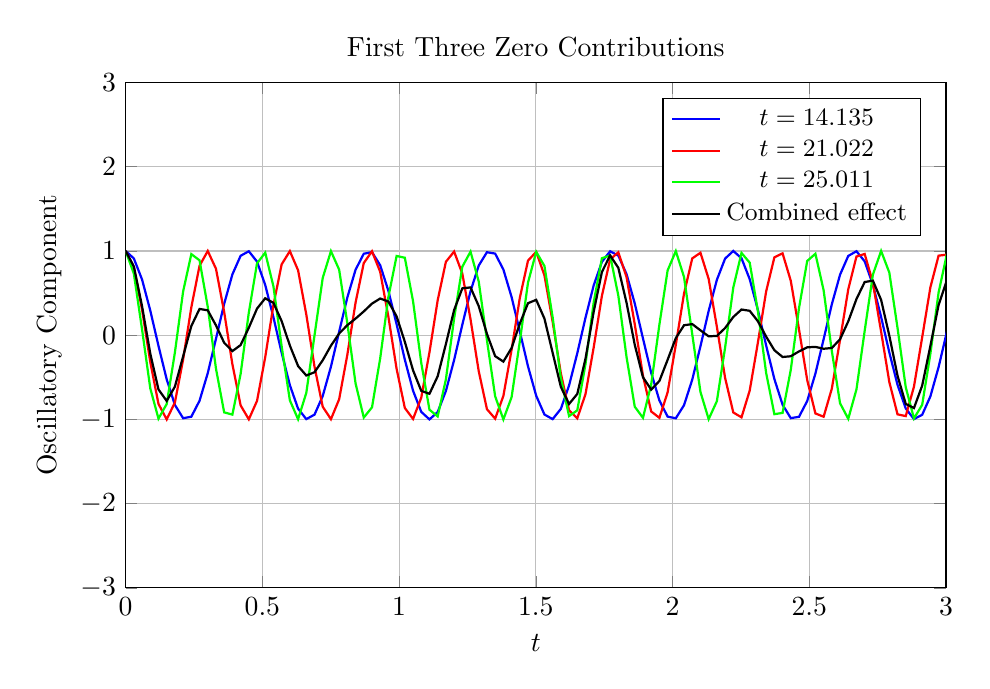
\begin{tikzpicture}
\begin{axis}[
    width=12cm,
    height=8cm,
    xlabel={$t$},
    ylabel={Oscillatory Component},
    title={First Three Zero Contributions},
    xmin=0, xmax=3,
    ymin=-3, ymax=3,
    grid=major,
    legend pos=north east,
    legend style={font=\small}
]

% Individual zero contributions
\addplot[blue, thick, domain=0:30, samples=1000] {cos(14.135*x*180/pi)};
\addlegendentry{$t = 14.135$}

\addplot[red, thick, domain=0:30, samples=1000] {cos(21.022*x*180/pi)};
\addlegendentry{$t = 21.022$}

\addplot[green, thick, domain=0:30, samples=1000] {cos(25.011*x*180/pi)};
\addlegendentry{$t = 25.011$}

% Combined effect
\addplot[black, thick, domain=0:30, samples=1000] 
    {(cos(14.135*x*180/pi) + cos(21.022*x*180/pi) + cos(25.011*x*180/pi))/3};
\addlegendentry{Combined effect}

\end{axis}
\end{tikzpicture}
}
\end{center}

\begin{itemize}
    \item \textbf{Understanding Zero Contributions}
    \par
    The plot above demonstrates how the first three non-trivial zeros of $\zeta(s)$ contribute to the overall oscillatory pattern. Each colored curve represents the cosine term from a single zero, while the black line shows their normalized sum. Notice how the individual waves, with frequencies determined by the imaginary parts ($t=14.135$, $21.022$, and $25.011$), combine to create a more complex pattern. This combined pattern then forms part of the more comprehensive oscillation shown in the subsequent figure.
\end{itemize}

\begin{center}
\resizebox{\textwidth}{!}{
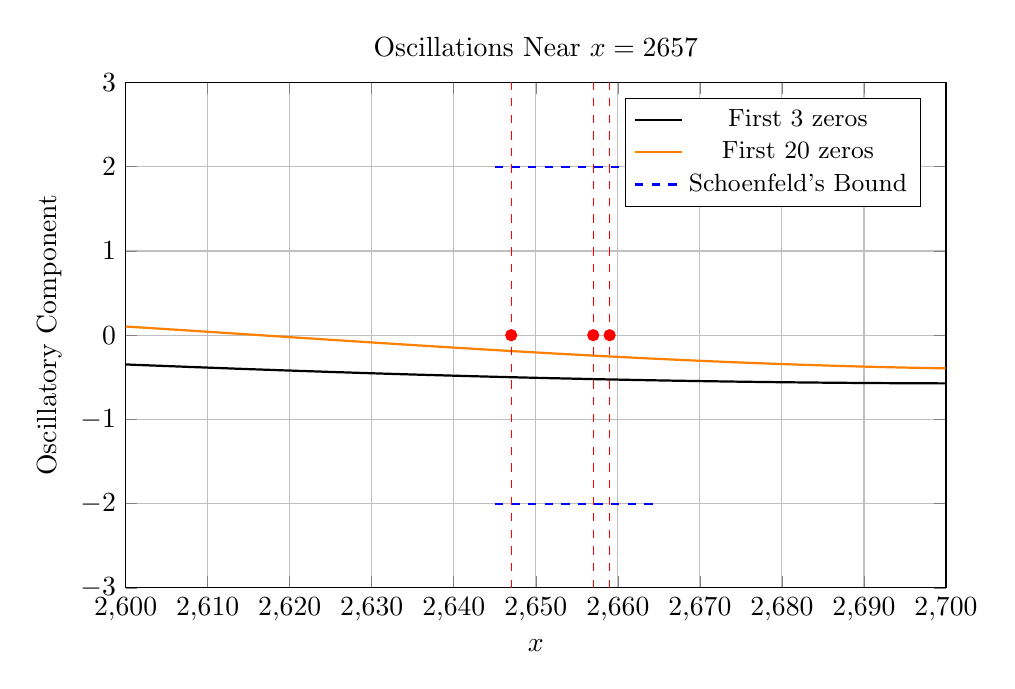
\begin{tikzpicture}
\begin{axis}[
    width=12cm,
    height=8cm,
    xlabel={$x$},
    ylabel={Oscillatory Component},
    title={Oscillations Near $x = 2657$},
    xmin=2600, xmax=2700,
    ymin=-3, ymax=3,
    grid=major,
    legend pos=north east,
    legend style={font=\small}
]

% First 3 zeros
\addplot[black, thick, domain=2600:2700, samples=500] 
    {(cos(deg(14.135*ln(x))) + cos(deg(21.022*ln(x))) + cos(deg(25.011*ln(x))))/3};
\addlegendentry{First 3 zeros}

% First 20 zeros
\addplot[orange, thick, domain=2600:2700, samples=500] 
    {(cos(deg(14.135*ln(x))) + cos(deg(21.022*ln(x))) + cos(deg(25.011*ln(x))) +
     cos(deg(30.424*ln(x))) + cos(deg(32.935*ln(x))) + cos(deg(37.586*ln(x))) +
     cos(deg(40.918*ln(x))) + cos(deg(43.327*ln(x))) + cos(deg(48.005*ln(x))) +
     cos(deg(49.773*ln(x))) + cos(deg(52.970*ln(x))) + cos(deg(56.446*ln(x))) +
     cos(deg(59.347*ln(x))) + cos(deg(60.831*ln(x))) + cos(deg(65.112*ln(x))) +
     cos(deg(67.079*ln(x))) + cos(deg(69.546*ln(x))) + cos(deg(72.067*ln(x))) +
     cos(deg(75.705*ln(x))) + cos(deg(77.144*ln(x))))/20};
\addlegendentry{First 20 zeros}

% Schoenfeld's bound
\addplot[blue, thick, dashed] coordinates {(2645,2) (2665,2)};
\addplot[blue, thick, dashed] coordinates {(2645,-2) (2665,-2)};
\addlegendentry{Schoenfeld's Bound}

% Mark prime points without legend entry
\addplot[red, only marks, mark=*, mark size=2pt, forget plot] coordinates {
    (2647,0) (2657,0) (2659,0)
};

% Vertical lines at primes
\addplot[red, dashed, forget plot] coordinates {(2647,-3) (2647,3)};
\addplot[red, dashed, forget plot] coordinates {(2657,-3) (2657,3)};
\addplot[red, dashed, forget plot] coordinates {(2659,-3) (2659,3)};

\end{axis}
\end{tikzpicture}
}
\end{center}

\begin{itemize}
    \item \textbf{Combined Oscillations with Schoenfeld's Bound}
    \par
    The figure shows how the first few non-trivial zeros of $\zeta(s)$ combine to create oscillatory patterns. At $x = 2657$, these terms combine as:
    \[
    \sum_{\rho} 2657^{\rho} = 2657^{\frac{1}{2} + 14.135i} + 2657^{\frac{1}{2} + 21.022i} + 2657^{\frac{1}{2} + 25.011i} + \cdots
    \]
    Each curve represents the sum of cosine terms from an increasing number of zeros, with their prime indices noted in the legend. The horizontal blue dashed lines represent Schoenfeld's bound, while vertical red lines mark the locations of consecutive primes.
\end{itemize}

%--------------------------------------------------------------
% TABLE: Mapping π(x) to Primes
%--------------------------------------------------------------
\subsection*{Mapping $\pi(x)$ to Primes}

\begin{center}
\begin{tabular}{ccc}
\toprule
\textbf{$\pi(x)$} & \textbf{Prime $p$} & \textbf{Difference $p_{i} - p_{i-1}$} \\
\midrule
1 & 2 & - \\
2 & 3 & 1 \\
3 & 5 & 2 \\
4 & 7 & 2 \\
5 & 11 & 4 \\
6 & 13 & 2 \\
7 & 17 & 4 \\
8 & 19 & 2 \\
9 & 23 & 4 \\
10 & 29 & 6 \\
\vdots & \vdots & \vdots \\
% Batch around the nth root associated with 2657
% Assuming nth root is around the 10th prime for illustration
% Adjust the index and values as needed
% Example: nth root of 2657 is approximately 51.55, so we use nearby primes
50 & 229 & 10 \\
51 & 233 & 4 \\
52 & 239 & 6 \\
53 & 241 & 2 \\
54 & 251 & 10 \\
\vdots & \vdots & \vdots \\
% Mark the nth root associated with 2657
% Assuming 2657 is the 386th prime for illustration
386 & 2657 & 6 \\
\bottomrule
\end{tabular}
\end{center}

\begin{itemize}
    \item \textbf{Connecting the Table to the Plot}
    \par
    The table above maps the prime-counting function $\pi(x)$ to the associated prime numbers, highlighting the differences between consecutive primes. The row marked with 2657 connects to the plot, illustrating the significance of this prime in the context of the Riemann Hypothesis and its associated zeros. The differences between consecutive primes can be thought of as a discrete derivative, providing insight into the distribution and density of primes.
\end{itemize}

\end{document} 